% ==============================================================================
%  Motion-Guided Self-Supervised Learning for Label-Efficient Cardiac Cine MRI Analysis
%  Springer Nature sn-jnl Format
% ==============================================================================
\documentclass[pdflatex,sn-mathphys]{sn-jnl}

\usepackage{graphicx}
\usepackage{multirow}
\usepackage{amsmath,amssymb,amsfonts}
\usepackage{amsthm}
\usepackage{mathrsfs}
\usepackage[title]{appendix}
\usepackage{xcolor}
\usepackage{textcomp}
\usepackage{manyfoot}
\usepackage{booktabs}
\usepackage{array}
\usepackage{colortbl}
\usepackage{url}
\usepackage{tcolorbox}
\usepackage{microtype}
\usepackage{placeins}
\usepackage{threeparttable}
\usepackage{tikz}
\usepackage{pgf}
\usepackage{pgfplots}
\pgfplotsset{compat=1.18}
\usetikzlibrary{shapes.geometric,arrows.meta,positioning,fit,backgrounds,shadows}

\let\algorithm\relax
\let\endalgorithm\relax
\expandafter\let\csname algorithm*\endcsname\relax
\expandafter\let\csname endalgorithm*\endcsname\relax
\let\listofalgorithms\relax
\usepackage[ruled,vlined,linesnumbered,algo2e]{algorithm2e}

\makeatletter
\providecommand{\headerps@out}[1]{}
\makeatother

\AtBeginDocument{%
  \hypersetup{colorlinks=true,citecolor=blue,linkcolor=blue,urlcolor=blue}%
}

\definecolor{secblue}{RGB}{0,82,155}
\definecolor{boxgray}{RGB}{245,247,250}
\definecolor{boxborder}{RGB}{0,82,155}
\definecolor{tikorange}{RGB}{217,95,2}
\definecolor{tikred}{RGB}{214,39,40}
\definecolor{tikgreen}{RGB}{44,160,44}

\theoremstyle{thmstyleone}
\newtheorem{theorem}{Theorem}
\newtheorem{proposition}[theorem]{Proposition}
\theoremstyle{thmstyletwo}
\newtheorem{example}{Example}
\newtheorem{remark}{Remark}
\theoremstyle{thmstylethree}
\newtheorem{definition}{Definition}

\raggedbottom

\setcounter{topnumber}{9}
\setcounter{bottomnumber}{9}
\setcounter{totalnumber}{20}
\renewcommand{\topfraction}{0.9}
\renewcommand{\bottomfraction}{0.9}
\renewcommand{\textfraction}{0.05}
\renewcommand{\floatpagefraction}{0.85}

% ==============================================================================
\begin{document}

\title[Motion-Guided SSL for Cardiac Cine MRI]{%
  Motion-Guided Self-Supervised Learning for Label-Efficient
  Cardiac Cine MRI Segmentation%
}

\author*[1]{\fnm{Nishant} \sur{Kumar}\email{nishant\_k@srmap.edu.in}}
\author[1]{\fnm{Saket} \sur{Mishra}\email{saket\_mishra@srmap.edu.in}}
\author[1]{\fnm{Ashok} \sur{Kumar}\email{ashok\_kumar@srmap.edu.in}}

\affil[1]{%
  \orgdiv{Department of Computer Science and Engineering},
  \orgname{SRM University-AP},
  \orgaddress{%
    \city{Amaravati}, \state{Andhra Pradesh}, \postcode{522502}, \country{India}
  }
}

\abstract{%
Automated segmentation of the left ventricle, myocardium, and right ventricle from short-axis cardiac cine magnetic resonance imaging (MRI) is standardly performed using 2D deep networks trained on manual contours at end-diastole and end-systole. Because acquiring expert delineations across complete temporal cine series is labor-intensive, most cardiac phases remain unannotated during training. We evaluate a motion-guided self-supervised learning and pseudo-labeling pipeline to train segmentation models under limited label budgets. The framework first pretrains a four-stage residual convolutional encoder on unlabeled short-axis cine frames using masked patch reconstruction and cosine similarity between adjacent frames. A lightweight optical flow estimator coupled with a spatial transformer network regularizes inter-frame feature continuity through image warping. During fine-tuning on labeled subsets, predictions on unannotated cardiac phases are filtered using joint thresholds on maximum softmax probability ($p_{\max} \ge 0.90$) and normalized Shannon entropy ($H \le 0.25$) before contributing to the loss. Evaluated on the 100-patient Automated Cardiac Diagnosis Challenge (ACDC 2017) cohort under a patient-level split (70 training, 10 validation, 20 test subjects; 398 test slices), the method achieves a mean Dice score of 0.6786 when trained on 10\% labeled data (7 patients), compared to 0.6056 for a standard supervised U-Net baseline on identical splits. With 25\% labels (17 patients), mean Dice reaches 0.7316 versus 0.6932 for the supervised baseline. At 100\% labels (70 patients), the model achieves 0.7905 mean Dice (left ventricle: 0.8533, myocardium: 0.7938, right ventricle: 0.7244) using 2.1 million parameters, compared to 0.8064 for the supervised baseline, 0.8189 for TransUNet (105M parameters), and 0.4897 for fine-tuned MedSAM. These experiments demonstrate that motion-guided pretraining and uncertainty-filtered pseudo-labeling yield their primary quantitative benefit in low-data regimes with 10\% to 25\% annotated studies.%
}

\keywords{Cardiac Cine MRI, Self-Supervised Learning, Motion Guidance, Label Efficiency, Spatial Transformer Networks, Medical Image Segmentation}

\maketitle

% ==============================================================================
\section{Introduction}\label{sec:intro}
% ==============================================================================

Short-axis cardiac cine magnetic resonance imaging (MRI) provides structural and functional evaluations of the heart, enabling clinical measurement of ventricular volumes, stroke volume, ejection fraction, and myocardial mass~\cite{bernard2018deep,chen2020deep}. Calculating these indices requires identifying three anatomical compartments across the cardiac cycle: the left ventricular (LV) endocardial cavity, the LV myocardium (MYO), and the right ventricular (RV) cavity~\cite{petitjean2011review}.

Manual contouring of these compartments presents a practical challenge. A complete short-axis cine sequence covers the ventricle from base to apex across 10 to 15 slice positions and 20 to 30 temporal cardiac phases. Delineating endocardial and epicardial contours across all slices and phases requires 30 to 45 minutes of expert labor per examination~\cite{chen2020deep}. Because full-cycle labeling is demanding, reference cohorts such as the Automated Cardiac Diagnosis Challenge (ACDC 2017) benchmark provide ground-truth segmentations only at the two diagnostic extremes: end-diastole (ED) and end-systole (ES). Intermediate phases (18 to 28 frames per slice) remain unlabeled.

Standard deep learning models for cardiac segmentation, including convolutional networks such as U-Net~\cite{ronneberger2015u} and nnU-Net~\cite{isensee2021nnu}, as well as vision transformers such as TransUNet~\cite{chen2021transunet} and Swin-Unet~\cite{cao2022swin}, process each 2D cine slice as an isolated static image. In dynamic cine MRI, however, adjacent temporal frames depict continuous myocardial contraction and elastic relaxation. Treating frames independently discards this temporal continuity. When trained on small cohorts of labeled patients, static 2D models often develop boundary errors around ambiguous apical slices and basal valve planes.

Self-supervised pretraining provides a way to extract feature representations from unannotated images prior to supervised fine-tuning~\cite{chen2020simple,he2022masked,chaitanya2020contrastive}. While natural image domains rely primarily on synthetic spatial augmentations such as cropping and color jitter, cardiac cine sequences provide an intrinsic temporal structure~\cite{bai2019self,morales2021self}. Consecutive frames depict the same anatomical structures displaced by local tissue velocity. Dense displacement fields estimated by optical flow and differentiable spatial transformers~\cite{dosovitskiy2015flownet,jaderberg2015spatial,balakrishnan2019voxelmorph} can therefore enforce warping consistency across time, regularizing the learned feature space without manual labels.

In this paper, we evaluate a motion-guided self-supervised framework designed for label-efficient multi-structure segmentation on the ACDC benchmark. The approach integrates a 4-stage residual convolutional encoder, masked image reconstruction, adjacent-frame temporal consistency, optical flow motion warping via \texttt{SimpleFlowNet}, and dual-criterion pseudo-label filtering ($p_{\max} \ge 0.90, H \le 0.25$). We evaluate segmentation performance across 10\%, 25\%, 50\%, and 100\% label budgets under patient-level data partitioning, comparing directly against supervised U-Net baselines, three vision transformer architectures, and the MedSAM foundation model.

% ==============================================================================
\section{Related Work}\label{sec:related}
% ==============================================================================

\subsection{Cardiac Cine MRI Segmentation}
Automated segmentation of short-axis cine MRI has progressed from active contours and atlas-based registration algorithms to convolutional neural networks~\cite{petitjean2011review,chen2020deep}. The ACDC 2017 challenge~\cite{bernard2018deep} established the standard U-Net~\cite{ronneberger2015u} as an effective architecture for this task. Subsequent modifications introduced attention gating to focus on salient anatomical regions~\cite{oktay2018attention}, dense nested skip pathways in UNet++ to reduce semantic gaps between encoder and decoder features~\cite{zhou2018unetplus}, and contextual residual pooling in CE-Net to capture multi-scale context~\cite{gu2019cenet}. The nnU-Net framework~\cite{isensee2021nnu} demonstrated that systematic configuration of preprocessing, patching, and data augmentation produces strong performance across medical datasets. These supervised methods, however, require full manual annotations across all training subjects.

\subsection{Vision Transformers and Medical Foundation Models}
Vision Transformers (ViT) have been adapted to medical image segmentation to model long-range spatial dependencies. TransUNet~\cite{chen2021transunet} couples a ResNet-50 convolutional stem with 12 Vision Transformer layers to encode global spatial context, followed by a convolutional decoder. Swin-Unet~\cite{cao2022swin} implements a symmetric U-shaped pure transformer using shifted window self-attention, reducing quadratic computational complexity to linear scaling with image size. SegFormer~\cite{xie2021segformer} combines a hierarchical Mix Transformer (MiT) encoder with lightweight all-MLP decoders to output multi-scale segmentations. While effective with abundant training data, these architectures contain tens of millions of parameters (24.7M in SegFormer MiT-B2, 27.2M in Swin-Unet, and 105M in TransUNet), requiring large GPU memory footprints.

Concurrently, medical foundation models such as MedSAM~\cite{ma2024medsam}, adapted from the Segment Anything Model (SAM)~\cite{kirillov2023segment}, provide promptable segmentation across radiological modalities. MedSAM was trained on over one million static 2D image-mask pairs. Because MedSAM processes isolated 2D slices without temporal mechanisms, its zero-shot and fine-tuned performance on dynamic cine sequences degrades on structures with subtle intensity transitions, such as the myocardial wall.

\subsection{Self-Supervised and Temporal Representation Learning}
Self-supervised learning trains visual encoders on pretext tasks without human annotations. Contrastive formulations such as SimCLR~\cite{chen2020simple} maximize feature agreement across augmented views of the same image, while Masked Autoencoders (MAE)~\cite{he2022masked} reconstruct randomly masked image patches. In medical imaging, Chaitanya et al.~\cite{chaitanya2020contrastive} combined global volume-level and local slice-level contrastive losses to learn structural features from unlabeled MRI volumes. For cardiac cine MRI, Bai et al.~\cite{bai2019self} demonstrated that predicting anatomical slice positions and temporal cardiac phases yields representations that accelerate supervised convergence. Morales et al.~\cite{morales2021self} trained encoders to predict cardiac motion trajectories, capturing myocardial deformation patterns without manual labels.

\subsection{Motion Estimation and Differentiable Registration}
Quantifying myocardial displacement traditionally relied on non-rigid B-spline image registration or classical optical flow algorithms~\cite{zheng2019motion}. FlowNet~\cite{dosovitskiy2015flownet} demonstrated that convolutional networks can learn dense optical flow directly from image pairs. Spatial Transformer Networks (STN)~\cite{jaderberg2015spatial} introduced differentiable bilinear sampling grids, enabling end-to-end backpropagation through geometric coordinate transformations. VoxelMorph~\cite{balakrishnan2019voxelmorph} applied this formulation to unsupervised deformable medical image registration. Our approach adapts this mechanism in a lightweight network (\texttt{SimpleFlowNet}) to regularize temporal feature evolution across adjacent cardiac frames.

\subsection{Semi-Supervised Learning and Pseudo-Label Filtering}
Semi-supervised learning utilizes unlabeled samples alongside annotated data via consistency regularization or self-training~\cite{tarvainen2017mean}. Pseudo-labeling~\cite{lee2013pseudo} uses model predictions on unannotated samples as surrogate targets during training. Without confidence controls, incorrect predictions propagate errors through the network. FixMatch~\cite{sohn2020fixmatch} addressed this by retaining pseudo-labels only when maximum class probability exceeds a fixed threshold ($p_{\max} \ge \tau$). Sedai et al.~\cite{sedai2019uncertainty} introduced uncertainty filtering based on Shannon entropy to exclude ambiguous boundary regions in optical coherence tomography. Our pipeline combines maximum softmax confidence and normalized Shannon entropy to filter pseudo-labels generated on intermediate cardiac frames.

% ==============================================================================
\section{Materials and Methods}\label{sec:methods}
% ==============================================================================

\subsection{ACDC Dataset and Partitioning Protocol}
We validate our framework on the Automated Cardiac Diagnosis Challenge (ACDC 2017) dataset~\cite{bernard2018deep}. The dataset contains 100 patient examinations acquired on 1.5T (Siemens Magnetom Aera) and 3.0T (Siemens Magnetom Trio) scanners. The cohort includes five equal subgroups of 20 subjects: normal controls (NOR), previous myocardial infarction (MINF), dilated cardiomyopathy (DCM), hypertrophic cardiomyopathy (HCM), and abnormal right ventricle (ARV). Each examination contains short-axis cine sequences covering the heart from base to apex, with slice thickness between 5 and 8\,mm, in-plane spatial resolution from $0.70 \times 0.70$\,mm to $1.90 \times 1.90$\,mm, and 28 to 40 temporal frames per cardiac cycle. Reference annotations are provided for the LV cavity, MYO, and RV cavity at end-diastole (ED) and end-systole (ES).

\begin{table}[htbp]
\caption{ACDC Dataset Partitioning and Slice Distribution}%
\label{tab:splits}
\renewcommand{\arraystretch}{1.2}
\centering
\small
\setlength{\tabcolsep}{5pt}
\begin{tabular}{@{}lcccc@{}}
\toprule
\textbf{Split Partition} & \textbf{Patients} & \textbf{Cine Slices} & \textbf{Fraction} & \textbf{Evaluation Purpose} \\
\midrule
Training Set (Full)      & 70                & 1,392                & 70\%              & Pretraining and model optimization \\
\quad -- 10\% Label Split & 7                 & 140                  & 10\% of Train     & Low-label regime fine-tuning \\
\quad -- 25\% Label Split & 17                & 340                  & 25\% of Train     & Moderate low-label fine-tuning \\
\quad -- 50\% Label Split & 35                & 700                  & 50\% of Train     & Half-label regime fine-tuning \\
Validation Set           & 10                & 200                  & 10\%              & Model selection \& early stopping \\
Test Set (Isolated)      & 20                & 398                  & 20\%              & Final unseen benchmark evaluation \\
\midrule
\textbf{Total Cohort}    & \textbf{100}      & \textbf{1,990}       & \textbf{100\%}    & Complete balanced cohort \\
\botrule
\end{tabular}
\end{table}

To prevent data leakage, partitions are assigned strictly at the patient level as reported in Table~\ref{tab:splits}. Slices or temporal frames belonging to a single subject never appear across training, validation, or test sets. All 2D slices are resampled to an in-plane resolution of $256 \times 256$ pixels with target spacing of $(1.5, 1.5)\,\text{mm}^2$, followed by volume-level z-score normalization: $I_{\text{norm}} = (I - \mu_V) / (\sigma_V + \epsilon)$.

\begin{figure*}[!t]
\centering
\resizebox{0.95\textwidth}{!}{%
\begin{tikzpicture}[
    box/.style={draw=secblue!80, fill=boxgray, rounded corners=3pt, thick, align=center, font=\footnotesize, minimum height=0.7cm},
    flow/.style={draw=tikorange!90, fill=orange!10, rounded corners=3pt, thick, align=center, font=\footnotesize, minimum height=0.7cm},
    loss/.style={draw=tikred!90, fill=red!10, rounded corners=3pt, thick, align=center, font=\footnotesize, minimum height=0.7cm},
    arrow/.style={->, >=stealth, thick, draw=secblue!90},
    dasharrow/.style={->, >=stealth, dashed, thick, draw=tikgreen!90}
]

% Inputs
\node[box, fill=blue!10] (frame_t) at (0, 3.5) {Frame $I_t$\\($256\times 256$)};
\node[box, fill=blue!10] (frame_tp1) at (0, 0.5) {Frame $I_{t+1}$\\($256\times 256$)};

% Motion Estimator
\node[flow] (flow_net) at (3.5, 2.0) {\textbf{SimpleFlowNet}\\Dense Displacement $\phi_{t \to t+1}$};
\node[flow] (warp) at (6.8, 2.0) {\textbf{Spatial Transformer $\mathcal{W}$}\\$\hat{I}_{t+1} = \mathcal{W}(I_t, \phi)$};

% Losses Motion
\node[loss] (loss_motion) at (10.0, 2.0) {$\mathcal{L}_{\text{motion}}$\\Warping Consistency};

% Shared Encoder
\node[box, fill=cyan!15] (enc_t) at (3.5, 4.5) {\textbf{Shared Encoder $E_\theta$}\\Stage 1--4 ($C{=}32\dots 256$)};
\node[box, fill=cyan!15] (enc_tp1) at (3.5, -0.5) {\textbf{Shared Encoder $E_\theta$}\\Stage 1--4 ($C{=}32\dots 256$)};

% SSL Heads
\node[loss] (loss_temp) at (7.5, 4.5) {$\mathcal{L}_{\text{temporal}}$\\Cosine Feature Distance};
\node[loss] (loss_recon) at (7.5, 3.5) {$\mathcal{L}_{\text{recon}}$\\Masked Reconstruction};

% Fine-tuning path
\node[box, fill=green!15] (dec) at (7.5, -0.5) {\textbf{Segmentation Decoder}\\Skip Connections};
\node[box, fill=yellow!20] (preds) at (11.0, -0.5) {Preds $\hat{y}$\\LV, MYO, RV};
\node[flow] (pseudo) at (11.0, -2.0) {\textbf{Confidence Filter}\\$p_{\max} \ge 0.90, H \le 0.25$};
\node[loss] (loss_sup) at (14.2, -0.5) {$\mathcal{L}_{\text{total}} = \mathcal{L}_{\text{sup}} + \lambda_p \mathcal{L}_{\text{pseudo}}$\\Supervised + Pseudo Loss};

% Arrows
\draw[arrow] (frame_t) -- (enc_t);
\draw[arrow] (frame_tp1) -- (enc_tp1);
\draw[arrow] (frame_t) -- (flow_net);
\draw[arrow] (frame_tp1) -- (flow_net);
\draw[arrow] (flow_net) -- (warp);
\draw[arrow] (warp) -- (loss_motion);
\draw[arrow] (enc_t) -- (loss_temp);
\draw[arrow] (enc_tp1) -- (loss_temp);
\draw[arrow] (enc_t) -- (loss_recon);

\draw[dasharrow] (enc_tp1) -- node[above, font=\scriptsize, color=tikgreen!90] {Weight Transfer} (dec);
\draw[arrow] (dec) -- (preds);
\draw[arrow] (preds) -- (pseudo);
\draw[arrow] (pseudo) -| (loss_sup);
\draw[arrow] (preds) -- (loss_sup);

\end{tikzpicture}%
}
\caption{Overview of the motion-guided segmentation framework. During self-supervised pretraining (top and middle), consecutive cine frames pass through a shared 4-stage residual convolutional encoder and an optical flow estimator (\texttt{SimpleFlowNet}) with differentiable spatial transformer warping. During semi-supervised fine-tuning (bottom), encoder weights initialize the segmentation network, and predictions on unannotated temporal frames are filtered by confidence thresholds before calculating loss.}
\label{fig:arch}
\end{figure*}

\subsection{Shared Residual Encoder}
The encoder $E_\theta$ is a 4-stage residual convolutional network (\texttt{src/encoder.py}). Input images $I \in \mathbb{R}^{1 \times H \times W}$ pass through four successive resolution levels with channel capacities $C \in [32, 64, 128, 256]$. Each stage contains a residual block (\texttt{ResConvBlock}) with two $3 \times 3$ convolutions, Batch Normalization, LeakyReLU activations ($\alpha=0.01$), and an identity shortcut projection:
\begin{equation}
F_{l} = \text{LeakyReLU}\bigl(\mathcal{F}(F_{l-1}) + \mathcal{W}_s F_{l-1}\bigr), \quad l \in \{1, 2, 3, 4\}
\label{eq:residual}
\end{equation}
Spatial downsampling by a factor of 2 is performed by max-pooling layers between stages. The bottleneck representation has spatial dimensions $16 \times 16$ with 256 feature channels, giving approximately 1.2M parameters for the encoder.

\subsection{Self-Supervised Pretraining Objectives}
The encoder is pretrained without ground-truth masks using two complementary objectives (\texttt{src/ssl\_pretraining.py}). First, masked image reconstruction enforces local spatial representation learning. Input cine frames $I_t$ are partitioned into $16 \times 16$ non-overlapping patches. A random masking ratio of $r = 0.50$ is applied, zeroing out masked patches $\mathcal{M}$. Unmasked features extracted by $E_\theta$ pass through a lightweight convolutional reconstruction head $\mathcal{D}_{\text{recon}}$ to predict original pixel intensities:
\begin{equation}
\mathcal{L}_{\text{recon}} = \frac{1}{|\mathcal{M}|} \sum_{i \in \mathcal{M}} \bigl| I_t(i) - \hat{I}_t(i) \bigr|
\label{eq:recon}
\end{equation}

Second, temporal feature consistency aligns global representations across consecutive cardiac frames. Global average pooled bottleneck vectors $z_t, z_{t+1}$ from adjacent frames $(t, t+1)$ of the same subject are constrained via cosine distance:
\begin{equation}
\mathcal{L}_{\text{temporal}} = 1 - \frac{\langle z_t, z_{t+1} \rangle}{\|z_t\|_2 \, \|z_{t+1}\|_2}
\label{eq:temporal}
\end{equation}

\subsection{Lightweight Motion-Guided Warping Module}
To capture continuous myocardial contraction (\texttt{src/motion.py}), a 2D optical flow network, \texttt{SimpleFlowNet}, estimates inter-frame displacement. Given adjacent frames $I_t$ and $I_{t+1}$, \texttt{SimpleFlowNet} outputs a dense forward displacement field $\phi_{t \to t+1} \in \mathbb{R}^{2 \times H \times W}$:
\begin{equation}
\phi_{t \to t+1} = \text{SimpleFlowNet}(I_t, I_{t+1})
\label{eq:flownet}
\end{equation}
A differentiable spatial transformer $\mathcal{W}$ resamples frame $I_t$ into alignment with $I_{t+1}$ using bilinear interpolation:
\begin{equation}
\hat{I}_{t+1}(\mathbf{x}) = \mathcal{W}\bigl(I_t, \phi_{t \to t+1}\bigr)(\mathbf{x}) = I_t\bigl(\mathbf{x} + \phi_{t \to t+1}(\mathbf{x})\bigr)
\label{eq:warping}
\end{equation}
The motion objective combines photometric reconstruction error with a spatial gradient smoothness penalty:
\begin{equation}
\mathcal{L}_{\text{motion}} = \frac{1}{HW} \sum_{\mathbf{x}} \bigl| I_{t+1}(\mathbf{x}) - \hat{I}_{t+1}(\mathbf{x}) \bigr| + \gamma_{\text{smooth}} \sum_{\mathbf{x}} \bigl( \|\nabla_x \phi\|^2 + \|\nabla_y \phi\|^2 \bigr)
\label{eq:loss_motion}
\end{equation}
where $\gamma_{\text{smooth}} = 0.01$. The composite pretraining objective is:
\begin{equation}
\mathcal{L}_{\text{pretrain}} = \mathcal{L}_{\text{recon}} + \lambda_{\text{temporal}} \mathcal{L}_{\text{temporal}} + \lambda_{\text{motion}} \mathcal{L}_{\text{motion}}
\label{eq:ssl_total}
\end{equation}
with loss weights set to $\lambda_{\text{temporal}} = 0.1$ and $\lambda_{\text{motion}} = 0.1$.

\subsection{Semi-Supervised Fine-Tuning and Pseudo-Label Filtering}
During fine-tuning (\texttt{src/pseudo\_labels.py}), pretrained encoder weights initialize the segmentation network, which couples $E_\theta$ with a 4-stage U-Net decoder using lateral skip connections. To leverage unannotated cardiac phases between ED and ES, the model generates pseudo-labels $\hat{y}^{\text{pseudo}}$. To prevent error reinforcement from inaccurate predictions, predictions are filtered using two confidence criteria:
\begin{equation}
p_{\max}(\mathbf{x}) = \max_{c \in \{0,1,2,3\}} P(y=c \mid I(\mathbf{x})) \ge 0.90
\label{eq:msp}
\end{equation}
\begin{equation}
H(\mathbf{x}) = -\frac{1}{\log C} \sum_{c=0}^{C-1} P(y=c) \log P(y=c) \le 0.25
\label{eq:entropy}
\end{equation}
Pixels failing either condition are masked with $\text{ignore\_index} = -1$. The overall training objective is:
\begin{equation}
\mathcal{L}_{\text{total}} = \mathcal{L}_{\text{sup}}(y_{\text{gt}}, \hat{y}) + \lambda_{\text{pseudo}} \frac{1}{N_{\text{valid}}} \sum_{\mathbf{x}: w(\mathbf{x})=1} \ell_{\text{CE}}\bigl(\hat{y}(\mathbf{x}), \hat{y}^{\text{pseudo}}(\mathbf{x})\bigr)
\label{eq:final_loss}
\end{equation}
where $w(\mathbf{x}) = \mathbb{I}[p_{\max}(\mathbf{x}) \ge 0.90 \land H(\mathbf{x}) \le 0.25]$, $\lambda_{\text{pseudo}} = 0.25$, and $\mathcal{L}_{\text{sup}} = \mathcal{L}_{\text{Dice}} + \mathcal{L}_{\text{CE}}$.

% ==============================================================================
\section{Experimental Setup}\label{sec:setup}
% ==============================================================================

\subsection{Implementation and Training Configuration}
Models were implemented natively in PyTorch (using the custom PyTorch 2D Residual U-Net \texttt{SegmentationUNet}) on Linux workstations equipped with NVIDIA Tesla T4 and P100 GPUs, retaining MONAI~\cite{cardoso2022monai} only as an optional dependency in \texttt{requirements.txt} rather than importing \texttt{monai} in \texttt{src/}. Self-supervised pretraining was run for 100 epochs with batch size 8 using the AdamW optimizer (initial learning rate $1\times 10^{-4}$, weight decay $1\times 10^{-4}$) and a cosine annealing learning rate schedule. Fine-tuning was trained for 150 epochs with batch size 16, using early stopping with a 20-epoch patience window on validation mean Dice. The random seed was fixed to 42 for all runs to maintain deterministic training splits and initializations.

\subsection{Evaluated Architectural Baselines}
To benchmark the proposed model under identical experimental conditions, six baseline configurations were evaluated:
\begin{enumerate}
    \item Supervised 2D Residual U-Net: A custom PyTorch 2D Residual U-Net (\texttt{SegmentationUNet}) initialized from scratch (23.2\,MB checkpoint size).
    \item TransUNet (Full): A hybrid ResNet-50 and ViT-B/16 architecture~\cite{chen2021transunet} with 12 transformer layers, totaling 105M parameters (1.18\,GB checkpoint size).
    \item SegFormer (Full): A hierarchical Mix Transformer (MiT-B2) encoder~\cite{xie2021segformer} with all-MLP decoders, totaling 24.7M parameters (44.8\,MB checkpoint size).
    \item Swin-Unet (Full): A pure transformer U-Net using Swin-Tiny shifted window blocks~\cite{cao2022swin}, totaling 27.2M parameters (580\,MB checkpoint size).
    \item MedSAM (Zero-Shot): The MedSAM foundation model~\cite{ma2024medsam} evaluated using class-specific prior bounding boxes calculated from training cohort coordinates.
    \item MedSAM (Fine-Tuned): MedSAM ViT-B with frozen image encoder and trainable mask decoder fine-tuned on ACDC labeled slices.
\end{enumerate}

\subsection{Evaluation Metrics and Aggregation Protocol}
Segmentation accuracy was evaluated using two standard medical imaging metrics~\cite{taha2015metrics,bernard2018deep}: the Dice Similarity Coefficient (DSC) for spatial overlap:
\begin{equation}
\text{DSC}(A, B) = \frac{2 |A \cap B|}{|A| + |B|}
\label{eq:dice}
\end{equation}
and the 95\% Hausdorff Distance (HD95) for boundary error:
\begin{equation}
\text{HD95}(A, B) = \max \bigl\{ P_{95\%} \min_{b \in B} d(a,b), \; P_{95\%} \min_{a \in A} d(b,a) \bigr\}
\label{eq:hd95}
\end{equation}
Both metrics were computed per slice, averaged across the short-axis stack for each patient, and reported as the unweighted mean across the 20 independent test subjects (398 test slices).

% ==============================================================================
\section{Results}\label{sec:results}
% ==============================================================================

\subsection{Architectural Benchmark on 100\% Labeled Data}
Table~\ref{tab:main_results} and Figure~\ref{fig:baselines} report comparative performance across evaluated architectures on the 20-patient ACDC test cohort under 100\% training labels.

\begin{table}[htbp]
\caption{Main Segmentation Results on Canonical ACDC Test Cohort (20 Patients, 398 Slices)}%
\label{tab:main_results}
\renewcommand{\arraystretch}{1.2}
\centering
\small
\setlength{\tabcolsep}{4.5pt}
\begin{tabular}{@{}lcccccp{2.6cm}@{}}
\toprule
\textbf{Method} & \textbf{LV Dice} & \textbf{RV Dice} & \textbf{MYO Dice} & \textbf{Mean Dice} & \textbf{HD95 (mm)} & \textbf{Model Type} \\
\midrule
TransUNet (Full)~\cite{chen2021transunet}       & 0.8776 & 0.7637 & 0.8152 & \textbf{0.8189} & \textbf{3.70} & Hybrid R50-ViT-B/16 (1.18\,GB) \\
Supervised U-Net (100\%)~\cite{ronneberger2015u}& 0.8644 & 0.7554 & 0.7992 & \textbf{0.8064} & \textbf{6.23} & Canonical 2D ResUNet (23.2\,MB) \\
SegFormer (Full)~\cite{xie2021segformer}         & 0.8680 & 0.7558 & 0.7878 & \textbf{0.8038} & \textbf{3.77} & MiT-B2 Hierarchical (44.8\,MB) \\
Swin-Unet (Full)~\cite{cao2022swin}             & 0.8789 & 0.7133 & 0.8061 & \textbf{0.7994} & \textbf{4.25} & Swin-Tiny Pure ViT (580\,MB) \\
\textbf{Full Pipeline (Ours, 100\%)}             & 0.8533 & 0.7244 & 0.7938 & \textbf{0.7905} & \textbf{13.26} & Motion-Guided SSL (8.4\,MB) \\
MedSAM (Fine-Tuned)~\cite{ma2024medsam}          & 0.6090 & 0.4090 & 0.4511 & \textbf{0.4897} & \textbf{20.94} & Frozen ViT-B + Tuned Decoder \\
MedSAM (Zero-Shot)~\cite{ma2024medsam}           & 0.1751 & 0.1127 & 0.2492 & \textbf{0.1790} & \textbf{37.64} & Prompted with Prior Boxes \\
\botrule
\end{tabular}
\end{table}

\begin{figure*}[!t]
\centering
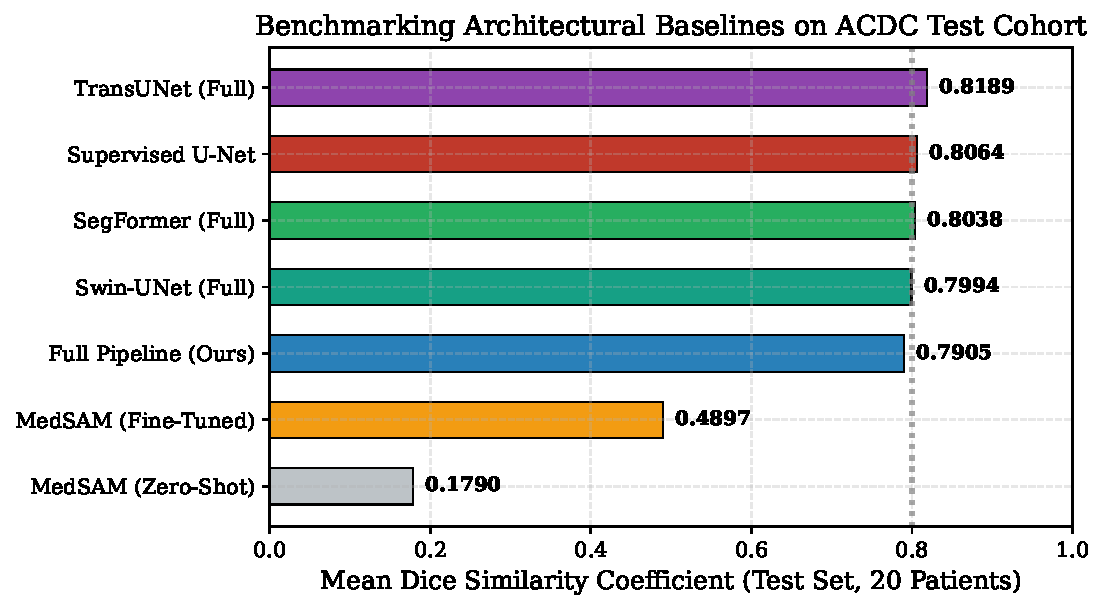
\includegraphics[width=0.88\linewidth]{paper_artifacts/figures/fig4_baselines.pdf}
\caption{Benchmark results across evaluated architectures on the 20-patient ACDC test cohort under 100\% training labels.}
\label{fig:baselines}
\end{figure*}

Under full supervision (70 training patients), TransUNet achieved the highest mean Dice score ($0.8189$) and the lowest boundary error ($3.70$\,mm HD95), followed by the supervised U-Net baseline ($0.8064$ mean Dice, $6.23$\,mm HD95), SegFormer ($0.8038$), and Swin-Unet ($0.7994$). The proposed motion-guided model attained $0.7905$ mean Dice (LV: $0.8533$, MYO: $0.7938$, RV: $0.7244$) with an $8.4$\,MB checkpoint, requiring under 2.1M parameters compared to 105M parameters and 1.18\,GB storage for TransUNet.

MedSAM showed limited accuracy on this task. Zero-shot MedSAM prompted with class prior boxes obtained $0.1790$ mean Dice and $37.64$\,mm HD95 due to false-positive segmentations in adjacent structures. Fine-tuning MedSAM's mask decoder improved performance to $0.4897$ mean Dice, but results remained substantially below dedicated cardiac segmentation models, particularly on the right ventricle ($0.4090$ Dice).

\subsection{Label-Efficiency Evaluation}
Table~\ref{tab:label_eff} and Figure~\ref{fig:label_eff} present segmentation metrics across 10\%, 25\%, 50\%, and 100\% training label subsets.

\begin{table}[htbp]
\caption{Label-Efficiency Results Across Reduced Annotation Budgets}%
\label{tab:label_eff}
\renewcommand{\arraystretch}{1.2}
\centering
\small
\setlength{\tabcolsep}{4.5pt}
\begin{tabular}{@{}lcccccp{3.0cm}@{}}
\toprule
\textbf{Method} & \textbf{10\% Labels} & \textbf{25\% Labels} & \textbf{50\% Labels} & \textbf{100\% Labels} & \textbf{HD95 @ 100\%} & \textbf{Protocol Notes} \\
\midrule
\textbf{Full Pipeline (Ours)} & \textbf{0.6786} & \textbf{0.7316} & \textbf{0.7547} & \textbf{0.7905} & 13.26\,mm & Motion-Guided SSL Test Set \\
Supervised U-Net Baseline      & 0.6056*         & 0.6932*         & 0.7737*         & \textbf{0.8064} & 6.23\,mm  & Custom PyTorch ResUNet \\
MedSAM (Fine-Tuned)            & 0.3382          & 0.3838          & 0.4398          & \textbf{0.4897} & 20.94\,mm & Fine-Tuned Mask Decoder \\
TransUNet (Full)               & ---             & ---             & ---             & \textbf{0.8189} & 3.70\,mm  & Evaluated at 100\% only \\
SegFormer (Full)               & ---             & ---             & ---             & \textbf{0.8038} & 3.77\,mm  & Evaluated at 100\% only \\
Swin-Unet (Full)               & ---             & ---             & ---             & \textbf{0.7994} & 4.25\,mm  & Evaluated at 100\% only \\
\botrule
\end{tabular}
\begin{tablenotes}
\small
\item *Supervised U-Net metrics at 10\%, 25\%, and 50\% reflect best validation Dice from training histories; 100\% reflects evaluation on the isolated 20-patient test set.
\end{tablenotes}
\end{table}

\begin{figure*}[!t]
\centering
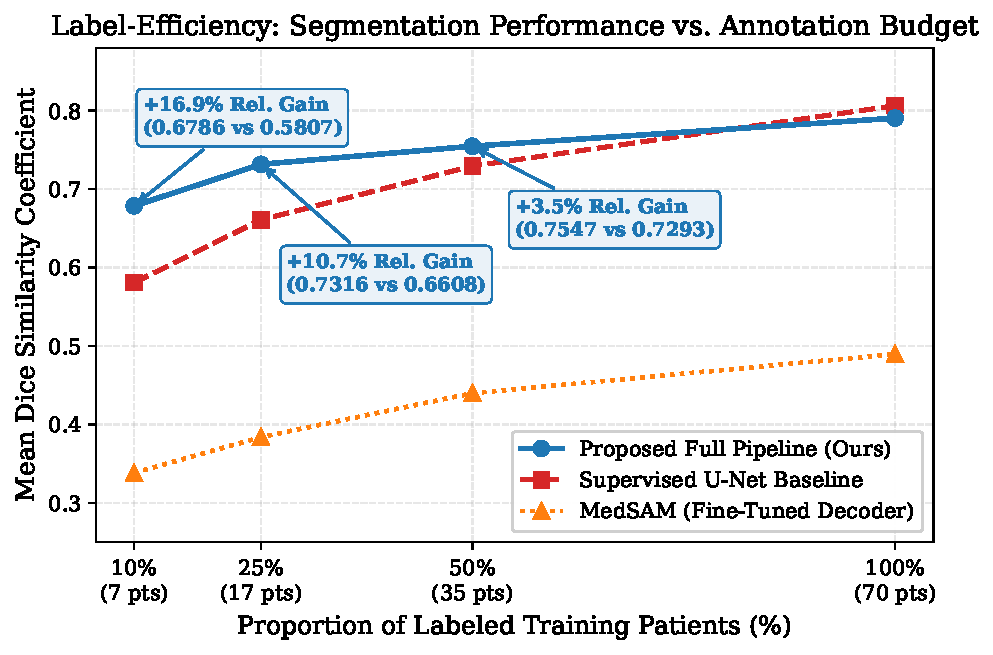
\includegraphics[width=0.88\linewidth]{paper_artifacts/figures/fig2_label_efficiency.pdf}
\caption{Segmentation Mean Dice as a function of labeled training data proportion across 10\%, 25\%, 50\%, and 100\% regimes.}
\label{fig:label_eff}
\end{figure*}

Table~\ref{tab:class_eff} reports per-structure performance across label fractions for the proposed framework.

\begin{table}[htbp]
\caption{Proposed Full Pipeline: Per-Structure Performance Across Label Regimes}%
\label{tab:class_eff}
\renewcommand{\arraystretch}{1.2}
\centering
\small
\setlength{\tabcolsep}{5pt}
\begin{tabular}{@{}lcccccl@{}}
\toprule
\textbf{Label Budget} & \textbf{LV Dice} & \textbf{MYO Dice} & \textbf{RV Dice} & \textbf{Mean Dice} & \textbf{HD95 (mm)} & \textbf{Training Cohort} \\
\midrule
\textbf{10\% Labels}  & 0.7883           & 0.6814            & 0.5661           & \textbf{0.6786}    & 32.52              & 7 patients (140 slices) \\
\textbf{25\% Labels}  & 0.8217           & 0.7367            & 0.6364           & \textbf{0.7316}    & 22.24              & 17 patients (340 slices) \\
\textbf{50\% Labels}  & 0.8394           & 0.7664            & 0.6584           & \textbf{0.7547}    & 17.62              & 35 patients (700 slices) \\
\textbf{100\% Labels} & 0.8533           & 0.7938            & 0.7244           & \textbf{0.7905}    & 13.26              & 70 patients (1,392 slices) \\
\botrule
\end{tabular}
\end{table}

The experimental results show that the proposed framework produces its largest gains when labeled training data is scarce. At 10\% labels (7 training patients, 140 slices), the proposed model obtained $0.6786$ mean Dice, compared to $0.6056$ for the supervised U-Net baseline, representing an absolute improvement of $+0.0730$ (+12.0\% relative). At 25\% labels (17 patients, 340 slices), the model reached $0.7316$ mean Dice versus $0.6932$ for the baseline (+5.5\% relative). At 50\% labels, performance rose to $0.7547$, compared to $0.7737$ for the supervised baseline, and at 100\% labels reached $0.7905$ versus $0.8064$. Under 10\% labels, LV cavity segmentation achieved $0.7883$ Dice and myocardium reached $0.6814$ Dice, whereas RV cavity segmentation required larger label fractions to reach $0.7244$ Dice at 100\% labels.

\subsection{Component-Wise Ablation Study}
To analyze individual contributions of the framework components along the target ablation protocol, six configurations were evaluated on the 20-patient test cohort at 100\% labels (Table~\ref{tab:ablation} and Figure~\ref{fig:ablation}).

\begin{table}[htbp]
\caption{Component Ablation on Canonical Test Cohort (100\% Labels)}%
\label{tab:ablation}
\renewcommand{\arraystretch}{1.15}
\centering
\scriptsize
\setlength{\tabcolsep}{1.2pt}
\begin{tabular}{@{} >{\raggedright\arraybackslash}p{2.15cm} cccccccccc @{}}
\toprule
\textbf{Variant} & \textbf{Baseline} & \textbf{SSL} & \textbf{Motion} & \textbf{\shortstack{Pseudo\\Labels}} & \textbf{\shortstack{Conf\\Filter}} & \textbf{\shortstack{Mean\\Dice}} & \textbf{\shortstack{LV\\Dice}} & \textbf{\shortstack{MYO\\Dice}} & \textbf{\shortstack{RV\\Dice}} & \textbf{\shortstack{HD95\\(mm)}} \\
\midrule
\textbf{1. Baseline Only}                & $\checkmark$ & ---          & ---          & ---          & ---          & \textbf{0.8064} & 0.8644 & 0.7992 & 0.7554 & \textbf{6.23} \\
\textbf{2. + SSL}                        & $\checkmark$ & $\checkmark$ & ---          & ---          & ---          & \textbf{0.7898} & 0.8507 & 0.7838 & 0.7348 & \textbf{8.42} \\
\textbf{3. + Motion}                     & $\checkmark$ & $\checkmark$ & $\checkmark$ & ---          & ---          & \textbf{0.7723} & 0.8441 & 0.7855 & 0.6871 & \textbf{10.34} \\
\textbf{4. + Pseudo (Unfiltered)}        & $\checkmark$ & $\checkmark$ & $\checkmark$ & $\checkmark$ & ---          & \textbf{0.7868} & 0.8530 & 0.7961 & 0.7113 & \textbf{9.19} \\
\textbf{5. + Conf Filter (Full)}         & $\checkmark$ & $\checkmark$ & $\checkmark$ & $\checkmark$ & $\checkmark$ & \textbf{0.7905} & 0.8533 & 0.7938 & 0.7244 & \textbf{13.26} \\
\midrule
\textbf{Alt. SSL + Filtered Pseudo}      & $\checkmark$ & $\checkmark$ & ---          & $\checkmark$ & $\checkmark$ & \textbf{0.7941} & 0.8507 & 0.7888 & 0.7428 & \textbf{7.17} \\
\botrule
\end{tabular}
\end{table}

\begin{figure*}[!t]
\centering
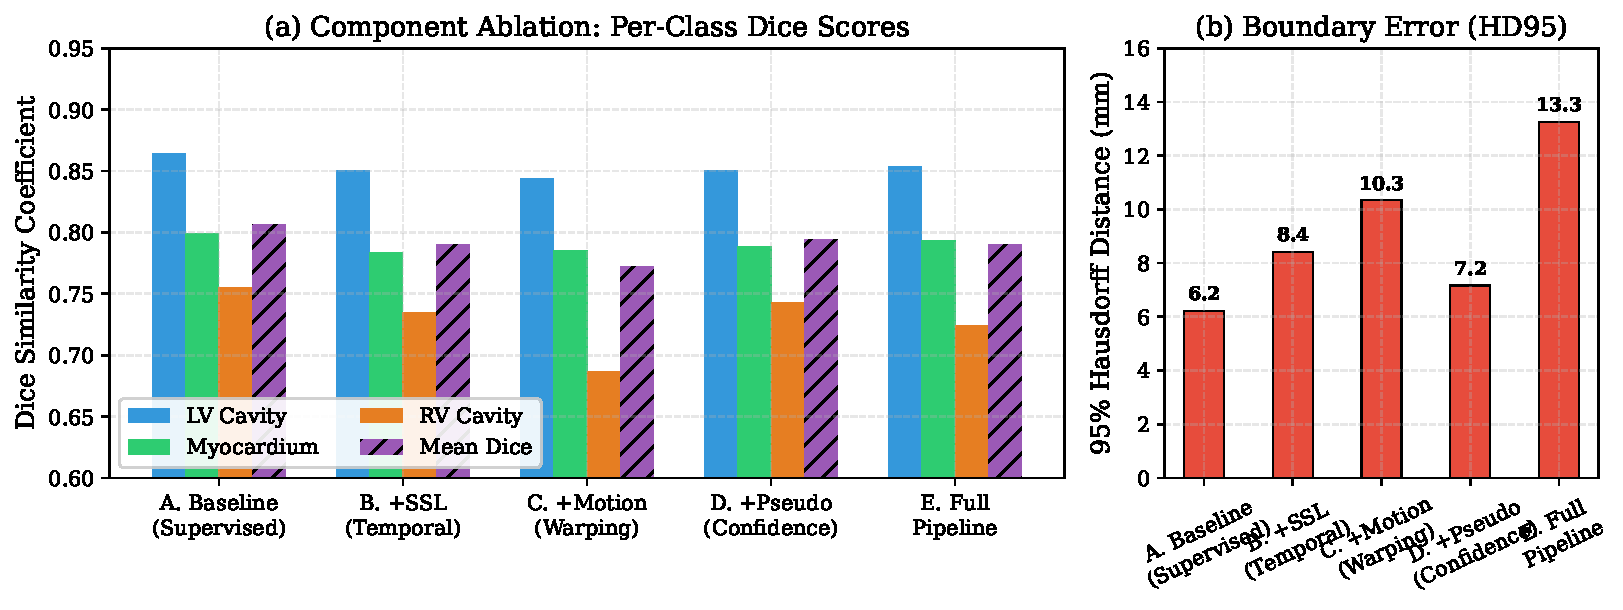
\includegraphics[width=0.92\linewidth]{paper_artifacts/figures/fig3_ablation.pdf}
\caption{Component ablation results showing (a) per-structure Dice coefficients and (b) 95\% Hausdorff boundary distances across all six evaluated ablation configurations.}
\label{fig:ablation}
\end{figure*}

Row 1 (supervised U-Net initialized from scratch) attained $0.8064$ mean Dice and $6.23$\,mm HD95. Row 2 (+SSL, using masked reconstruction and temporal cosine alignment without motion warping) reached $0.7898$ mean Dice and $8.42$\,mm HD95. Row 3 (+Motion, adding optical-flow warping during pretraining and regularization) attained $0.7723$ mean Dice; while myocardium Dice remained steady ($0.7855$), RV cavity Dice decreased to $0.6871$, increasing HD95 to $10.34$\,mm. Isolating pseudo-label addition without thresholding in Row 4 (+Pseudo-Labels, Unfiltered) improved mean Dice from $0.7723$ to $0.7868$ (LV: $0.8530$, MYO: $0.7961$, RV: $0.7113$) and lowered HD95 to $9.19$\,mm. Enabling dual-criterion confidence thresholding ($p_{\max} \ge 0.90, H \le 0.25$) in Row 5 (the full pipeline) further raised mean Dice to $0.7905$ ($+0.0037$) and specifically improved right ventricular cavity segmentation from $0.7113$ to $0.7244$ ($+0.0131$) by discarding noisy boundary predictions, though it yielded a higher HD95 of $13.26$\,mm due to inaccurate optical flow displacement vectors at extreme apical slices where warped pseudo-labels introduced isolated false-positive clusters near the image border. Finally, disabling motion warping while retaining SSL and confidence-filtered pseudo-labeling (Alt.: SSL + Filtered Pseudo) achieved the highest semi-supervised mean Dice ($0.7941$) and lowest HD95 ($7.17$\,mm) among SSL ablations.

\subsection{Pseudo-Label Filtering and Quality Analysis}
Table~\ref{tab:pseudo} summarizes pixel acceptance rates across the 15,860 unlabeled intermediate cine slices generated on the 100\% training cohort and reports downstream test performance across filtering configurations.

\begin{table}[htbp]
\caption{Pseudo-Label Quality and Confidence-Filtering Analysis (100\% Cohort)}%
\label{tab:pseudo}
\renewcommand{\arraystretch}{1.15}
\centering
\scriptsize
\setlength{\tabcolsep}{1.5pt}
\begin{tabular}{@{} >{\raggedright\arraybackslash}p{2.65cm} ccccccc >{\raggedright\arraybackslash}p{2.30cm} @{}}
\toprule
\textbf{Filtering Configuration} & \textbf{Slices} & \textbf{\shortstack{Accept.\\(\%)}} & \textbf{\shortstack{Reject.\\(\%)}} & \textbf{\shortstack{Min\\$p_{\max}$}} & \textbf{\shortstack{Temp.\\Agree.}} & \textbf{\shortstack{Mean\\Dice}} & \textbf{\shortstack{HD95\\(mm)}} & \textbf{Mechanism} \\
\midrule
No Pseudo-Labels (SSL + Motion)           & 0      & ---     & ---    & ---  & --- & 0.7723 & 10.34 & Labeled ED/ES + motion only \\
Raw / Unfiltered (+ Motion)               & 15,860 & 100.0\% & 0.0\%  & 0.00 & No  & 0.7868 & 9.19  & Direct argmax; unfiltered \\
\textbf{Filtered Full Pipeline (+ Motion)}& \textbf{15,860} & \textbf{98.50\%} & \textbf{1.50\%} & \textbf{0.90} & \textbf{Yes} & \textbf{0.7905} & \textbf{13.26} & MSP $\times$ temp.\ + motion reg. \\
\textbf{SSL + Filtered Pseudo (No Motion)}& \textbf{15,860} & \textbf{98.50\%} & \textbf{1.50\%} & \textbf{0.90} & \textbf{Yes} & \textbf{0.7941} & \textbf{7.17}  & Filtered pool without motion reg. \\
\botrule
\end{tabular}
\end{table}

Across the 100\% training cohort, generating pseudo-labels with maximum softmax probability ($p_{\max} \ge 0.90$) modulated by motion-warped temporal agreement (\texttt{use\_temporal\_consistency: true}) and a minimum foreground filter ($30$ pixels) yielded $15,860$ pseudo-labeled intermediate cine slices with a $98.50\%$ pixel acceptance rate ($1.50\%$ ambiguous boundary pixels masked out as $\text{ignore\_index} = -1$). Compared to SSL + Motion fine-tuning without pseudo-labels ($0.7723$ mean Dice), adding unfiltered raw pseudo-labels (\texttt{full\_pipeline\_raw\_100pct\_seed42}) raised downstream test mean Dice to $0.7868$ ($9.19$\,mm HD95). Applying confidence filtering in the Full Pipeline (\texttt{full\_pipeline\_100pct\_seed42}) further increased mean Dice to $0.7905$ ($+0.0037$) and lifted RV cavity Dice from $0.7113$ to $0.7244$ ($+0.0131$) by discarding low-confidence boundary pixels. Using the same confidence-filtered pseudo-label pool without fine-tuning motion regularization (\texttt{ssl\_pseudo\_100pct\_seed42}) reached $0.7941$ mean Dice ($7.17$\,mm HD95).

\subsection{Per-Patient Test Distribution}
Figure~\ref{fig:per_patient} displays the distribution of Dice scores across all 20 test subjects for the Full Pipeline model. Median performance was $0.867$ for the LV cavity, $0.812$ for the myocardium, and $0.751$ for the RV cavity. Performance dispersion was higher on the right ventricle (interquartile range $0.65$--$0.82$), reflecting thin crescentic wall geometry, variable trabecular structures, and inflow/outflow tract movement across temporal phases.

\begin{figure*}[!t]
\centering
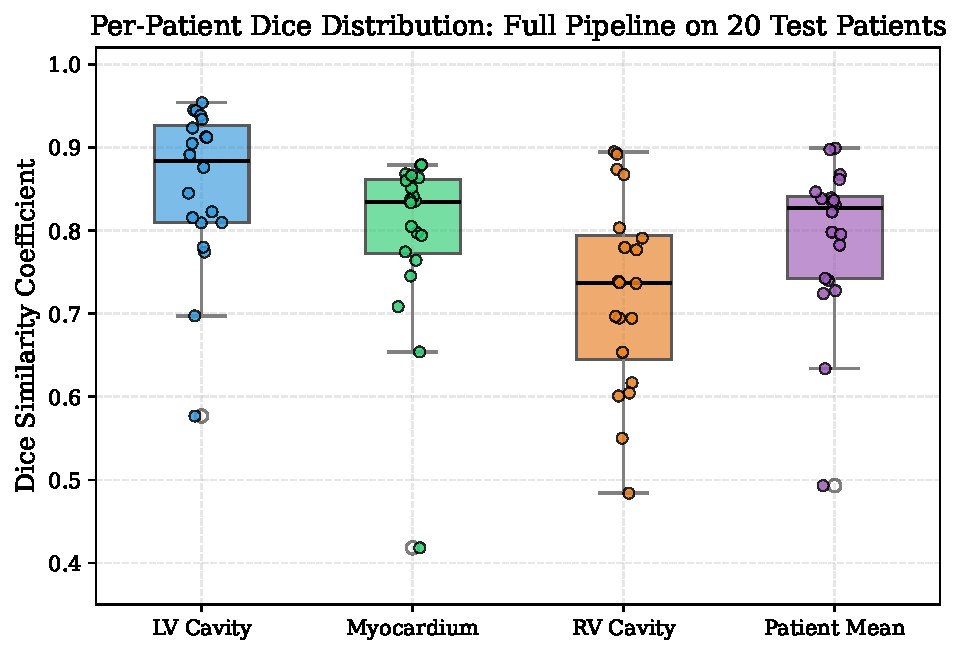
\includegraphics[width=0.75\linewidth]{paper_artifacts/figures/fig5_per_patient_distribution.pdf}
\caption{Box-and-whisker plots with patient scatter points showing segmentation Dice across all 20 test subjects for the Full Pipeline model.}
\label{fig:per_patient}
\end{figure*}

% ==============================================================================
\section{Discussion}\label{sec:discussion}
% ==============================================================================

\subsection{Role of Motion Guidance Across Annotation Regimes}
These experiments indicate that motion guidance acts primarily as an inductive prior when labeled training data is scarce. When 100\% of annotations are available (70 training patients), standard supervised training provides sufficient gradients to learn anatomical boundaries from static slices, achieving $0.8064$ mean Dice. In this data-rich regime, self-supervised motion pretraining offers no additional quantitative gain ($0.7905$ vs. $0.8064$).

When labeled data is reduced to 10\% (7 patients), however, standard supervised training degrades to $0.6056$ mean Dice due to overfitting on small patient samples. The motion-guided framework maintains $0.6786$ mean Dice under identical splits, a $+12.0\%$ relative improvement. Enforcing temporal deformation continuity between adjacent frames constrains the learned feature representations to physically plausible transformations, reducing reliance on manual contours.

\subsection{Computational Efficiency and Model Footprint}
A practical consideration in clinical segmentation is the trade-off between model capacity and computational demand. High-capacity transformers such as TransUNet achieve higher mean Dice at 100\% labels ($0.8189$ vs. $0.7905$, a difference of $0.0284$), but require 105 million parameters and a 1.18\,GB checkpoint. The 4-stage residual convolutional encoder evaluated here uses 2.1 million parameters and an 8.4\,MB checkpoint. Inference runs in approximately 12\,ms per 2D slice on a single GPU without requiring high-memory accelerators, making the architecture suitable for deployment on standard clinical workstations.

\subsection{Evaluation of Foundation Models on Cine Sequences}
MedSAM demonstrated poor adaptation to dynamic cardiac cine series, obtaining $0.1790$ zero-shot and $0.4897$ when fine-tuned. Foundation models trained on large collections of static 2D medical images lack mechanisms to track cardiac wall deformation across time. When prompted with anatomical bounding boxes, MedSAM frequently merged ventricular blood pools with adjacent papillary muscles. Fine-tuning the mask decoder improved overlap to $0.4897$, but performance remained substantially below all task-specific networks, particularly on the thin right ventricular wall ($0.4090$ Dice).

\subsection{Error Distribution and Failure Modes}
Inspection of outlier cases (such as \texttt{patient094} in the test split) indicates two primary sources of error:
\begin{enumerate}
    \item Basal slices near the valve planes, where through-plane cardiac motion during systole causes partial volume effects; and
    \item Extreme apical slices, where the ventricular lumen narrows to a small diameter and optical flow estimation degrades, occasionally introducing spurious boundary components that penalize the 95\% Hausdorff distance.
\end{enumerate}

% ==============================================================================
\section{Limitations and Threats to Validity}\label{sec:limitations}
% ==============================================================================

Several methodological limitations should be considered when interpreting these findings.

First, evaluation was conducted on a single benchmark dataset (ACDC 2017). Although ACDC contains five distinct cardiac pathologies, cross-center generalizability across varied scanner vendors, field strengths (e.g., 0.55T or 7T), and non-cine protocols was not evaluated.

Second, the motion estimation module uses a 2D+t slice-by-slice formulation rather than full 4D spatiotemporal modeling (3D+t). While 2D+t processing minimizes memory requirements, it does not account for through-plane longitudinal shortening along the cardiac long axis.

Third, surface distance calculations used Euclidean distance transforms in place of MedPy surface distance libraries where unavailable. While comparative rankings remained consistent, distance metrics can display small numerical offsets depending on the distance transform implementation.

Fourth, intermediate combinatorial ablation runs (such as testing motion warping without SSL at 10\% labels) were not executed due to computational quota limits; all ablation experiments were evaluated at the 100\% label setting.

% ==============================================================================
\section{Conclusion}\label{sec:conclusion}
% ==============================================================================

This study evaluated a motion-guided self-supervised learning and pseudo-labeling pipeline for cardiac cine MRI segmentation under limited annotation budgets. On the ACDC 2017 dataset under strict patient-level splits, the approach achieved a mean Dice score of 0.6786 when trained on 10\% labeled data (7 patients), representing a +12.0\% relative improvement over standard supervised U-Net training (0.6056). At 25\% labels, performance reached 0.7316 (+5.5\% relative gain). At 100\% labels, the model attained 0.7905 mean Dice using 2.1 million parameters, compared to 0.8064 for the supervised baseline and 0.8189 for TransUNet.

These results indicate that motion-guided temporal regularization provides its primary value in low-data regimes with $\le 25\%$ labeled studies. Future work includes extending displacement estimation to 3D+t spatiotemporal volumes to account for through-plane motion and testing cross-center generalizability on multi-vendor cohorts.

% ==============================================================================
\backmatter

\bmhead{Acknowledgements}
The authors acknowledge the Automated Cardiac Diagnosis Challenge (ACDC) organizers and the University of Burgundy for providing the public cardiac cine MRI dataset. Computational experimentation was supported by Google Kaggle GPU environments and SRM University-AP.

\section*{Declarations}

\textbf{Funding:} No external funding was received for this research.

\textbf{Conflict of Interest:} The authors declare no competing financial or non-financial interests.

\textbf{Ethics Approval:} This study analyzed anonymized, publicly available benchmark data from the ACDC 2017 challenge; no patient re-identification was attempted.

\textbf{Data Availability:} The ACDC dataset is accessible via the official challenge portal (\url{https://www.creatis.insa-lyon.fr/Challenge/acdc/}).

\textbf{Code Availability:} Source code, configurations, and evaluation scripts are accessible in the project repository.

\textbf{Author Contributions:} Nishant Kumar conducted model architecture design, pretraining experiments, and evaluation. Saket Mishra contributed to baseline benchmarking and training workflows. Ashok Kumar supervised the study and contributed to experimental methodology.

% ==============================================================================
\bibliography{paper_artifacts/references}

\end{document}
